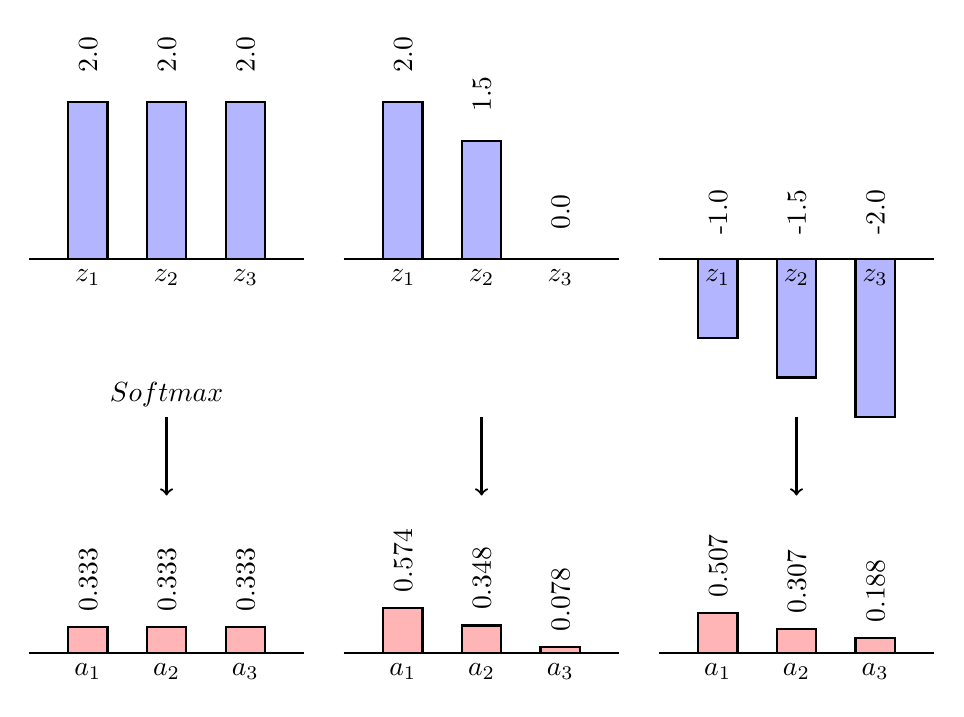
\begin{tikzpicture}[thick]
	\definecolor{incolor}{RGB}{180, 181, 255}
	\definecolor{outcolor}{RGB}{255, 181, 181}
	
	% \drawcol#x#y#value#label#color
	\def\drawcol#1#2#3#4#5{
		\filldraw[fill=#5] (#1, {min(#2, #2 + #3)}) rectangle (#1 + .5, {max(#2, #2 + #3)}) 
			node[above, rotate=90, xshift=6mm] {#3};
		\node[anchor=north] at (#1 + .25, #2) {#4};
	}

	% \drawbar#x#y#value1#value2#value3#label#color
	\def\drawbar#1#2#3#4#5#6#7{
		\draw (#1, #2) -- (#1 + 3.5, #2);
		\drawcol{#1 + 0.5}{#2}{#3}{$#6_1$}{#7}
		\drawcol{#1 + 1.5}{#2}{#4}{$#6_2$}{#7}
		\drawcol{#1 + 2.5}{#2}{#5}{$#6_3$}{#7}
	}
	
	% input
	\drawbar{0}{5} { 2.0}{ 2.0}{ 2.0} {z} {incolor}
	\drawbar{4}{5} { 2.0}{ 1.5}{ 0.0} {z} {incolor}
	\drawbar{8}{5} {-1.0}{-1.5}{-2.0} {z} {incolor}
	
	% down arrow
	\draw[->] (1.75, 3) node[above] {$Softmax$} -- (1.75, 2) ;
	\draw[->] (5.75, 3) -- (5.75, 2);
	\draw[->] (9.75, 3) -- (9.75, 2);
	
	% output
	\drawbar{0}{0} {0.333}{0.333}{0.333} {a} {outcolor}
	\drawbar{4}{0} {0.574}{0.348}{0.078} {a} {outcolor}
	\drawbar{8}{0} {0.507}{0.307}{0.188} {a} {outcolor}
\end{tikzpicture}